% EURS AI Studio -- paper draft.
% Build:  cd paper && latexmk -pdf main.tex   (or: pdflatex main; bibtex main; pdflatex main; pdflatex main)
% Tables in generated/ and figures in figures/ are written by ml/make_report.py. Do not edit them by hand.
% Before submission: switch to the official WACV/MaCVi template, fill author info, resolve every \todo{}.
\documentclass[10pt,twocolumn,letterpaper]{article}
\usepackage[margin=0.75in,columnsep=0.3125in]{geometry}
\usepackage{times}
\usepackage[T1]{fontenc}
\usepackage{microtype}
\usepackage{amsmath,amssymb}
\usepackage{graphicx}
\usepackage{booktabs}
\usepackage{multirow}
\usepackage[table]{xcolor}
\usepackage[font=small,labelfont=bf]{caption}
\usepackage[numbers,sort&compress]{natbib}
\usepackage[colorlinks=true,citecolor=blue!60!black,linkcolor=blue!60!black,urlcolor=blue!60!black]{hyperref}
\usepackage[capitalise,noabbrev]{cleveref}

% Draft markers. Set \drafttrue -> \draftfalse to check nothing is left (all \todo will error).
\newif\ifdraft \drafttrue
\ifdraft
  \newcommand{\todo}[1]{{\color{red!75!black}\textbf{[TODO: #1]}}}
\else
  \newcommand{\todo}[1]{\errmessage{Unresolved TODO: #1}}
\fi
\newcommand{\ours}{EURS-Net}
\newcommand{\lite}{EURS-Lite}

\title{\Large\bf Restoration-Aware Segmentation of Underwater Imagery\\for the EURS Challenge}
\author{\todo{Author One}\textsuperscript{1} \quad \todo{Author Two}\textsuperscript{1}\\
\textsuperscript{1}\todo{Affiliation}\\
{\small\tt\todo{email}}}
\date{}

\begin{document}
\maketitle

\begin{abstract}
Water absorbs red light first and scatters a blue-green veil over every scene, so the two things a marine
survey needs from a camera, faithful colour and reliable scene parsing, degrade together. We study underwater
image restoration and five-class semantic segmentation (background, coral, fish, elasmobranch, other)
jointly on the EURS benchmark. We propose \ours{}, a single network with a shared encoder and two decoders, in
which features of the restoration decoder are fused into the segmentation decoder at every scale
(restoration-to-segmentation, R2S, fusion). We also release \lite{}, a CPU-only baseline built from two
small per-pixel networks that trains in minutes, and an open protocol for both tasks: a split of the official
training data grouped by dive so that near-duplicate frames cannot leak across splits, model selection on
validation data only, and a single scored pass on a held-out test split with bootstrap confidence intervals.
On the held-out EURS test split, \ours{} reaches \todo{X.XX}\,dB PSNR and \todo{XX.X}\% mIoU, compared with
\todo{X.XX}\,dB and \todo{XX.X}\% for a classical colour-correction and threshold baseline.
Code, trained models and an interactive demo are available at
\url{https://github.com/nvaltryek-001/EURS-ai-studio}.
\end{abstract}

% =====================================================================================
\section{Introduction}
Cameras on divers, remotely operated vehicles and autonomous underwater vehicles are now a routine instrument
for reef monitoring, fisheries assessment and the study of protected species such as sharks and rays.
Two properties of water make their images hard to use. Wavelength-dependent attenuation removes red, then green,
light with distance, and back-scattered ambient light adds a range-dependent veil~\cite{jaffe1990computer,
mcglamery1980computer,akkaynak2018revised}. The result is low contrast and a strong blue-green cast that both
misleads human annotators and shifts the input distribution of recognition models trained in air.

Restoration and recognition have mostly been studied apart: enhancement methods are judged by image-quality
metrics~\cite{li2020uieb,islam2020funie,liu2020ruie}, and segmentation benchmarks such as SUIM~\cite{islam2020suim}
evaluate parsing on unrestored inputs. The EURS challenge~\cite{eurs2027challenge}, part of the MaCVi
workshop series~\cite{kiefer2025macvi}, couples the two: participants restore degraded underwater images and
segment them into five marine classes. This raises a practical question that we study directly: \emph{should a
segmenter see the restored image, the degraded image, or a shared representation of both?}

\paragraph{Contributions.}
\begin{itemize}\setlength\itemsep{1pt}
  \item \textbf{\ours{}}, a dual-decoder network whose segmentation decoder receives restoration features at
        every scale (R2S fusion), trained with a multi-task objective that tolerates samples lacking either label.
  \item \textbf{\lite{}}, a training-light baseline (two small per-pixel MLPs on colour-statistics and texture
        features) that runs in NumPy on a CPU, giving a reproducible lower bound and a fallback for embedded use.
  \item \textbf{A leakage-aware protocol} for EURS: a dive-grouped, rare-class-stratified 80/10/10 split of the
        official training archive; validation-only model selection; and test-split reporting with per-class IoU
        and bootstrap confidence intervals. The split files and evaluation code are released.
  \item An open-source web studio and API that serves the trained models for interactive inspection.
\end{itemize}

% =====================================================================================
\section{Related Work}
\paragraph{Underwater image formation and restoration.}
Physics-based models describe an observed channel $I_c$ as the scene radiance $J_c$ attenuated by transmission
$t_c$ plus back-scatter $B_c$~\cite{jaffe1990computer,mcglamery1980computer}; Akkaynak and
Treibitz~\cite{akkaynak2018revised} showed that the attenuation coefficients governing direct and back-scattered
light differ, and Sea-thru~\cite{akkaynak2019seathru} inverts the revised model given range. Prior-based methods
adapt the dark channel prior from dehazing~\cite{he2011dark}, while classical colour constancy (gray-world
\cite{buchsbaum1980spatial}) and local contrast enhancement (CLAHE~\cite{zuiderveld1994clahe}) remain common,
training-free baselines. Learned enhancement became practical with paired benchmarks such as UIEB~\cite{li2020uieb}
and fast networks such as FUnIE-GAN~\cite{islam2020funie}. Because clean references are rarely available,
no-reference measures such as UCIQE~\cite{yang2015uciqe} and UIQM~\cite{panetta2016uiqm} are widely reported.

\paragraph{Underwater semantic segmentation.}
SUIM~\cite{islam2020suim} introduced a pixel-level benchmark for underwater scenes and showed that standard
encoder--decoder architectures such as U-Net~\cite{ronneberger2015unet} transfer reasonably but suffer on thin
and rare classes. Rare classes are a recurring difficulty: elasmobranchs occupy a small fraction of pixels and
of images, which motivates class-balanced losses~\cite{milletari2016vnet} and stratified evaluation.

\paragraph{Joint restoration and recognition.}
Multi-task learning shares representations across tasks and can be sensitive to loss weighting
\cite{kendall2018multitask}. In the MaCVi 2025 underwater restoration challenge, the winning entry reported that its two-stage
restoration pipeline improved downstream detection of marine species~\cite{kiefer2025macvi}. Our R2S fusion takes the
next step of letting segmentation consume restoration features inside one network, rather than chaining two
separately trained models.

% =====================================================================================
\section{Method}
\subsection{Problem setting}
Given a degraded RGB image $x\in[0,1]^{H\times W\times 3}$, we predict a restored image $\hat y$ and a label map
$\hat m\in\{0,\dots,4\}^{H\times W}$ for the classes background, coral, fish, elasmobranch and other. Training
samples may provide a clean reference $y$, a mask $m$, or both; the losses below are masked accordingly.

\subsection{\lite{}: a CPU baseline}
\lite{} is two-stage. \emph{Restoration:} for each pixel we compute a 23-dimensional descriptor of colour and
local statistics (RGB; Gaussian means and standard deviations at $\sigma\in\{6,24\}$; image-level channel means
and standard deviations; a $15{\times}15$ dark channel~\cite{he2011dark}; and normalised row position, a proxy
for range in typical down-looking and horizontal views). An MLP regresses the \emph{residual} $y-x$, which is
low-frequency; we predict it at a working resolution of at most 384\,px, upsample it, and add it to the
full-resolution input so fine detail is preserved. \emph{Segmentation:} a second MLP classifies each pixel of the
restored image from colour (RGB, Lab, HSV with circular hue), multi-scale context (Lab means and luminance
standard deviation at $\sigma\in\{2,6,16\}$), texture (gradient magnitude and Laplacian at two scales) and row
position. Class probabilities are spatially smoothed before the arg-max. Both MLPs are trained on class-balanced
pixel samples from the training split; hidden sizes and the smoothing scale are chosen on the validation split.
Weights are exported to a plain array file, and inference needs only NumPy and OpenCV.

\subsection{\ours{}: dual decoders with R2S fusion}
\paragraph{Architecture.} A shared encoder (ResNet-18~\cite{he2016resnet} or MobileNetV3-Large~\cite{howard2019mobilenetv3},
ImageNet-initialised, with input normalisation folded into the graph) produces features $F_1,\dots,F_5$ at strides
2 to 32. Two U-Net-style decoders~\cite{ronneberger2015unet} upsample with skip connections. Let $R_k$ be the
restoration decoder's output at scale $k$. The segmentation decoder block at the same scale receives
\begin{equation}
S_k = \phi_k\big([\,\mathrm{up}(S_{k-1}),\; F_{5-k},\; R_k\,]\big),
\end{equation}
where $[\cdot]$ is channel concatenation and $\phi_k$ two conv--BN--ReLU layers. The restoration head predicts a
bounded residual, $\hat y=\mathrm{clip}\big(x+\tanh(h_r([\,\mathrm{up}(R_4),x\,])),0,1\big)$, and the segmentation head
predicts logits $\hat z=h_s(S_4)$ upsampled to full resolution. Because $R_k$ is used by the segmentation branch,
the segmentation loss also shapes the restoration features.

\paragraph{Objective.} With $\mathbb{1}_y,\mathbb{1}_m$ indicating label availability,
\begin{align}
\mathcal{L} &= \lambda_r\,\mathbb{1}_y\big(\lVert\hat y-y\rVert_1 + \alpha\,(1-\mathrm{SSIM}(\hat y,y))\big) \nonumber\\
&\;+ \lambda_s\,\mathbb{1}_m\big(\mathrm{CE}_w(\hat z,m) + \beta\,\mathcal{L}_{\mathrm{Dice}}(\hat z,m)\big),
\end{align}
where $\mathrm{CE}_w$ is cross-entropy with class weights $w_c\propto f_c^{-1/2}$ ($f_c$ the training pixel frequency,
normalised to mean one and capped at $10\times$ the smallest), $\mathcal{L}_{\mathrm{Dice}}$ the soft Dice
loss~\cite{milletari2016vnet} over classes present in the batch, and pixels labelled \emph{ignore} are excluded. We
use $\lambda_r=\lambda_s=1$, $\alpha=0.2$, $\beta=0.5$.

% =====================================================================================
\section{Experimental Protocol}
\subsection{Data and splits}
We use the official EURS training archive~\cite{eurs2027challenge}. The development archive contains degraded images
only; it is never used for training or model selection and serves only to produce challenge submissions.
Because consecutive frames from one dive are near duplicates, a random image-level split would place almost identical
images in training and test sets and inflate scores. We therefore group images by sequence identifier (the filename
prefix before the frame number) and split \emph{groups} 80/10/10 into train, validation and test, stratifying on the
rarest class each group contains. \Cref{tab:split} summarises the result. \todo{State how sequence ids are encoded in
the EURS filenames, and confirm the grouping heuristic matches it.}

\begin{table}[t]
\centering\small
\begin{tabular}{lcccc}\toprule Split & Train & Val & Test & Total \\ \midrule Images & -- & -- & -- & -- \\ \bottomrule\end{tabular}

\caption{Dive-grouped split of the EURS training archive (seed 2027).}
\label{tab:split}
\end{table}

\subsection{Metrics}
\emph{Restoration:} PSNR and SSIM~\cite{wang2004ssim} against the clean reference (8-bit RGB, data range 255),
and the no-reference UCIQE~\cite{yang2015uciqe}. \emph{Segmentation:} a confusion matrix accumulated over all test
pixels, from which we report per-class IoU, mean IoU over classes present in the ground truth, mean F1, precision and
recall. \emph{Uncertainty:} 95\% confidence intervals from 1{,}000 bootstrap resamples of test
\emph{images}~\cite{efron1993bootstrap}, recomputing dataset-level mIoU for each resample. \emph{Cost:} median
end-to-end CPU latency per image, including pre- and post-processing. \todo{Add the official EURS challenge metric if it
differs, and report the leaderboard score of the dev-set submission.}

\subsection{Baselines and implementation}
\emph{Classical:} gray-world white balance~\cite{buchsbaum1980spatial}, CLAHE on Lab
luminance~\cite{zuiderveld1994clahe} and a bilateral filter, followed by a colour-threshold segmentation heuristic.
\emph{Identity:} the degraded input scored against the reference. \lite{} uses scikit-learn MLPs (Adam, early
stopping on held-out training pixels). \ours{} is trained with AdamW~\cite{loshchilov2019adamw} (learning rate
$3\times10^{-4}$, weight decay $10^{-4}$, linear warm-up then cosine decay), batch size 8, random scaled crops of
$384^2$ with horizontal flips, mixed precision, for up to 60 epochs with early stopping (patience 15) on the
validation score $\mathrm{mIoU}+\mathrm{PSNR}/40$. Inference resizes to $512^2$ and re-injects full-resolution detail by
upsampling the predicted correction. \todo{GPU model and wall-clock training time.}

% =====================================================================================
\section{Results}
\begin{table*}[t]
\centering\small
\begin{tabular}{lccccccc}
\toprule
Method & PSNR$\uparrow$ & SSIM$\uparrow$ & UCIQE$\uparrow$ & mIoU (\%)$\uparrow$ & mF1 (\%)$\uparrow$ & EURS$^{\approx}\uparrow$ & ms/img$\downarrow$ \\
\midrule
Degraded input (identity) & -- & -- & -- & -- & -- & -- & -- \\
Classical (GW+CLAHE / heuristic) & -- & -- & -- & -- & -- & -- & -- \\
EURS-Lite (ours, CPU) & -- & -- & -- & -- & -- & -- & -- \\
EURS-Net-Tiny (ours, embedded) & -- & -- & -- & -- & -- & -- & -- \\
EURS-Net (ours, ResNet-18) & -- & -- & -- & -- & -- & -- & -- \\
\bottomrule
\end{tabular}

\caption{Held-out EURS test split. Brackets: 95\% bootstrap confidence intervals over test images. Latency is the
median per image on CPU for the full pipeline.}
\label{tab:main}
\end{table*}

\begin{table*}[t]
\centering\small
\begin{tabular}{lcccccc}
\toprule
Method & Background & Coral & Fish & Elasmobranch & Other & mIoU \\
\midrule
Classical (GW+CLAHE / heuristic) & -- & -- & -- & -- & -- & -- \\
EURS-Lite (ours, CPU) & -- & -- & -- & -- & -- & -- \\
EURS-Net-Tiny (ours, embedded) & -- & -- & -- & -- & -- & -- \\
EURS-Net (ours, ResNet-18) & -- & -- & -- & -- & -- & -- \\
\bottomrule
\end{tabular}

\caption{Per-class IoU (\%) on the held-out EURS test split.}
\label{tab:perclass}
\end{table*}

\Cref{tab:main} compares all methods on the held-out test split and \cref{tab:perclass} breaks segmentation down by
class. \todo{Describe the main findings once the numbers exist: the restoration gain over the identity and classical
baselines, the mIoU gap between \lite{} and \ours{}, and whether the confidence intervals overlap.}
\todo{Discuss the elasmobranch class specifically: its pixel share in \cref{tab:split}, its IoU, and the dominant
confusions in \cref{fig:confusion}.}

\begin{figure}[t]
\centering
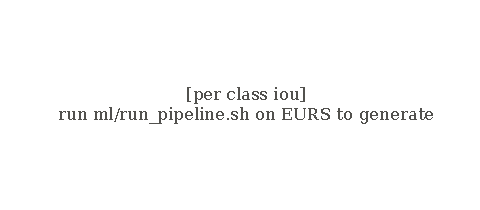
\includegraphics[width=\linewidth]{figures/main_per_class_iou.pdf}
\caption{Per-class IoU on the EURS test split.}
\label{fig:perclass}
\end{figure}

\begin{figure}[t]
\centering
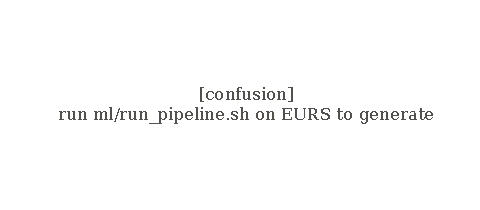
\includegraphics[width=0.85\linewidth]{figures/main_confusion.pdf}
\caption{Row-normalised confusion matrix of the best model on the EURS test split.}
\label{fig:confusion}
\end{figure}

\begin{figure*}[t]
\centering
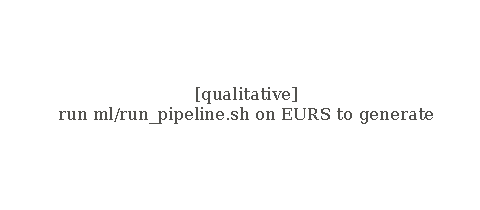
\includegraphics[width=\linewidth]{figures/main_qualitative.pdf}
\caption{Qualitative results on EURS test images.}
\label{fig:qual}
\end{figure*}

\subsection{Ablations}
\begin{table}[t]
\centering\small
\resizebox{\linewidth}{!}{\begin{tabular}{lccc}
\toprule
Variant & PSNR$\uparrow$ & SSIM$\uparrow$ & mIoU (\%)$\uparrow$ \\
\midrule
Full EURS-Net (ResNet-18, R2S fusion) & -- & -- & -- \\
w/o R2S fusion & -- & -- & -- \\
MobileNetV3-L encoder & -- & -- & -- \\
Segmentation only ($\lambda_r{=}0$) & -- & -- & -- \\
Restoration only ($\lambda_s{=}0$) & -- & -- & -- \\
\bottomrule
\end{tabular}
}
\caption{Ablations of \ours{} on the EURS test split.}
\label{tab:ablation}
\end{table}
\Cref{tab:ablation} isolates the design choices: removing R2S fusion, replacing the encoder with MobileNetV3-Large
for embedded deployment, and training each task alone. \todo{Interpret: does fusion help segmentation, does the
joint loss help or hurt restoration, and what is the accuracy cost of the MobileNet encoder?}

\begin{figure*}[t]
\centering
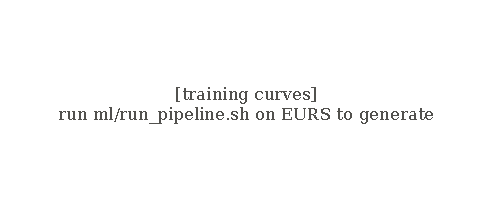
\includegraphics[width=\linewidth]{figures/main_training_curves.pdf}
\caption{Training dynamics. Left: training (solid) and validation (dashed) loss. Right: validation score per epoch.}
\label{fig:curves}
\end{figure*}

% =====================================================================================
\section{Limitations}
PSNR and SSIM require clean references whose own fidelity is unknown for real underwater scenes, so we also report a
no-reference score; neither fully captures perceived quality or scientific usefulness. Our split is internal to the
official training archive and may be easier than the challenge's hidden test data if the latter comes from different
sites or cameras. The sequence-grouping heuristic depends on filename conventions. \lite{} classifies pixels
independently apart from probability smoothing, which limits it on thin and small objects.

\section{Conclusion}
We presented a joint restoration and segmentation model for underwater imagery, a CPU baseline, and a leakage-aware
evaluation protocol for EURS. \todo{One-sentence summary of the headline result.} All code, split files, trained
weights and the interactive studio are public.

{\small
\bibliographystyle{unsrtnat}
\bibliography{refs}
}

% =====================================================================================
\clearpage
\appendix
\section{Pipeline Verification on Synthetic Data}
\label{app:synthetic}
\emph{The numbers in this appendix are not EURS results.} To check the full pipeline (indexing, splitting, training,
evaluation and reporting) independently of the official data, we render 300 procedural reef scenes with
pixel-exact five-class masks and degrade them with the image formation model
$I_c = J_c\,t_c + B_c(1-t_c)$, $t_c=e^{-\beta_c z}$~\cite{akkaynak2018revised}, with randomly drawn
attenuation coefficients ($\beta_R>\beta_G\gtrsim\beta_B$), back-scatter colour, range maps, artificial lighting,
forward-scatter blur and sensor noise. Frames are generated in groups of six that share a ``dive'' prefix so that the
grouped split is exercised. \Cref{tab:syn} and \cref{fig:syn-qual} show that \lite{} learns both tasks on this data,
whereas the classical pipeline does not. Because the degradation model is known and the scenes are simple, these
scores are far higher than should be expected on real imagery.

\begin{table*}[h]
\centering\small
\begin{tabular}{lccccccc}
\toprule
Method & PSNR$\uparrow$ & SSIM$\uparrow$ & UCIQE$\uparrow$ & mIoU (\%)$\uparrow$ & mF1 (\%)$\uparrow$ & EURS$^{\approx}\uparrow$ & ms/img$\downarrow$ \\
\midrule
Degraded input (identity) & 9.99 & 0.636 & 0.149 & -- & -- & -- & -- \\
Classical (GW+CLAHE / heuristic) & 12.19\,{\scriptsize[11.8, 12.6]} & 0.681 & 0.169 & 7.0\,{\scriptsize[5.9, 8.3]} & 15.3 & 0.143 & 4.1 \\
EURS-Lite (ours, CPU) & 29.56\,{\scriptsize[28.9, 30.1]} & 0.859 & 0.180 & 79.2\,{\scriptsize[75.2, 83.0]} & 87.5 & 0.683 & 167.5 \\
\bottomrule
\end{tabular}

\caption{Synthetic sanity check (test split of 30 images; not EURS data).}
\label{tab:syn}
\end{table*}

\begin{figure*}[h]
\centering
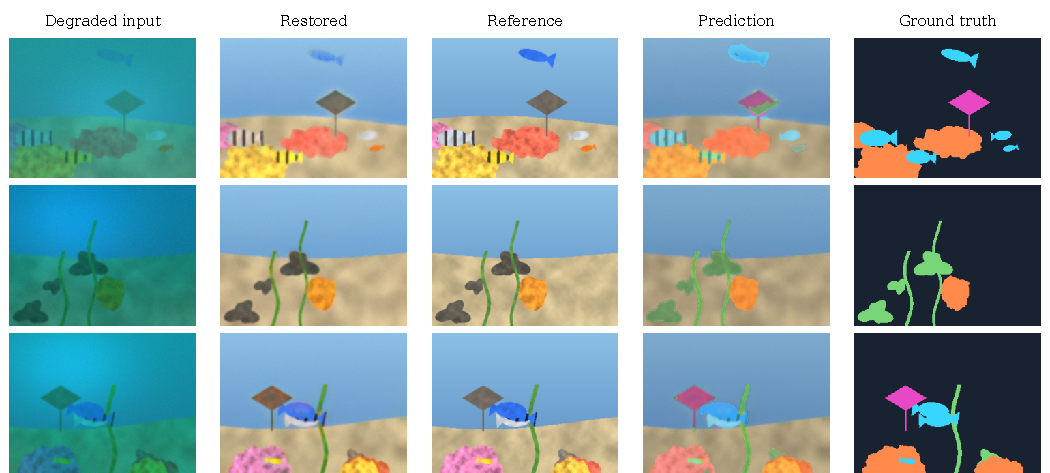
\includegraphics[width=0.9\linewidth]{figures/synthetic_qualitative.pdf}
\caption{Synthetic test scenes: degraded input, \lite{} restoration, clean reference, predicted labels over the
restored image, and ground truth.}
\label{fig:syn-qual}
\end{figure*}

\begin{figure}[h]
\centering
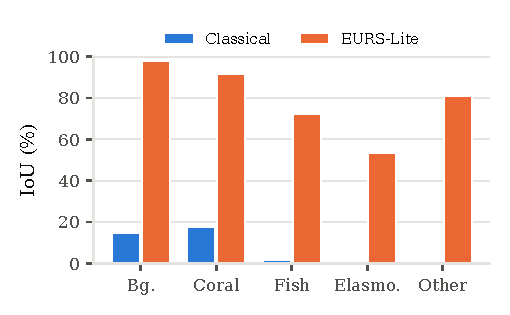
\includegraphics[width=\linewidth]{figures/synthetic_per_class_iou.pdf}
\caption{Per-class IoU on the synthetic test split.}
\end{figure}

\end{document}
